\documentclass[aspectratio=1610]{beamer}
% --------------------------------------------------
% Opções para "aspectratio"
% 43 ou 54: Formatos 4:3 ou 5:4 tradicionais para telas antigas
% 169, 1610 ou 189: Formatos 16:9, 16:10 ou 18:9 widescrenn telas mais modernas
% --------------------------------------------------
\usepackage{ifslides2024} % Tema (não remover)
\usepackage{lipsum}       % Gerador de texto dummy
\usepackage{csquotes}
\usepackage[utf8]{inputenc}

\addbibresource{referencias.bib} % Referências
% Dados da Apresentação
\titulo{Predição do Ganho Médio Diário de Peso em Bovinos de Corte via Redes Neurais Artificiais}
\subtitulo{Seminário de Qualificação de TCC}
\autor{Euler Gomes da Rocha}
\email{eulergomesrocha@gmail.com}
\info{% Informações adicionais (opcional)
  Bacharelado em Engenharia de Computação \\%
  \textbf{Orientador:} Prof. Dr. Ciniro Aparecido Leite Nametala \\
  \textbf{Coorientadora:} Dra. Tamires Martins Rezende
}
\campus{Bambuí}
\data{2026}

\begin{document}

% Página inicial
\begin{frame}[plain, fragile]
  \titlepage
\end{frame}

% ------------------------------------------------------------

% Sumário
\begin{frame}[fragile]{Sumário}
  \tableofcontents
\end{frame}

% ------------------------------------------------------------

\section{Introdução}


\subsection{Contextualização}

\begin{frame}[fragile] \frametitle{Introdução -- Contextualização}
	\begin{itemize} \itemsep0.8em
	  \item Pecuária de corte: o Brasil é um dos maiores produtores e exportadores mundiais \cite{usda2026}. O agronegócio fechou 2025 com exportações recordes de US\$ 169 bi e superávit de US\$ 149 bi \cite{ministerio2026}.

	  \item O Ganho Médio Diário (GMD) é um dos principais indicadores de desempenho produtivo -- o acréscimo médio de peso corporal por dia de avaliação \cite{embrapa2026}:
	  $$GMD = (peso\_atual - peso\_anterior) / dias\_entre\_pesagens$$

    \item Sua predição é complexa: resulta da interação de múltiplos fatores -- genéticos, nutricionais, sanitários, climáticos e de manejo \cite{tambara2021, faria2025, alencastrofilho2017}.

    \item Redes Neurais Artificiais (RNA) modelam relações não lineares a partir de dados históricos \cite{silva2016, goodfellow2016}.

	\end{itemize}
\end{frame}

% ------------------------------------------------------------

\subsection{Objetivos}

\begin{frame}[fragile] \frametitle{Introdução -- Objetivos}
\begin{block}{Objetivo Geral}
  Desenvolver e validar um modelo de Rede Neural Artificial (MLP) para a predição do GMD em bovinos de corte da microrregião de Bambuí-MG, a partir de variáveis zootécnicas, nutricionais, sanitárias, climáticas e de manejo, classificando os animais em categorias de desempenho produtivo com base nas estimativas obtidas.
\end{block}
\vskip1em
\begin{block}{Objetivos Específicos}
  \begin{enumerate}
		\item Coletar e consolidar os dados das propriedades rurais
		\item Realizar o pré-processamento e a análise exploratória dos dados
		\item Desenvolver e treinar o modelo de RNA (MLP) para predição do GMD
		\item Converter as estimativas de GMD em categorias de desempenho produtivo
		\item Avaliar o desempenho do modelo por métricas estatísticas (MSE, RMSE, MAE)
  \end{enumerate}
\end{block}
\end{frame}

% ------------------------------------------------------------

\subsection{Justificativa}

\begin{frame}[fragile] \frametitle{Introdução -- Justificativa}
\begin{itemize} \itemsep0.8em
\item O GMD é um dos principais indicadores de desempenho na pecuária de corte \cite{alencastrofilho2017}, mas sua predição é complexa e os modelos tradicionais têm limitações na captura de relações não lineares \cite{faria2025}.

\item As RNAs permitem modelar essas relações com maior precisão \cite{silva2016, goodfellow2016}.

\item \textbf{Lacuna:} em pesquisa preliminar na base Scopus, não foram encontrados trabalhos com esse recorte regional e essa combinação de variáveis.

\item \textbf{Diferencial:} integra variáveis zootécnicas, sanitárias, climáticas e de manejo obtidas por registros de rotina -- sem dependência de equipamentos de alto custo (câmeras/sensores).

\item \textbf{Aplicação:} ferramenta de apoio à decisão acessível a produtores de pequeno e médio porte.
\end{itemize}
\end{frame}

% ------------------------------------------------------------

\subsection{Classificação da pesquisa}

\begin{frame}[fragile] \frametitle{Introdução -- Classificação da pesquisa}
\begin{itemize} \itemsep1em
\item Natureza: Aplicada, uma vez que tem como objetivo o desenvolvimento de uma solução tecnológica com aplicação prática no contexto da pecuária de corte.

\item Abordagem: Quantitativa, uma vez que se baseia na análise de dados numéricos e na aplicação de técnicas estatísticas e computacionais para modelagem e predição do fenômeno estudado.

\item Objetivo: Explicativo, pois busca identificar e compreender as relações entre variáveis zootécnicas, ambientais e de manejo que influenciam o ganho de peso dos bovinos.

\item Procedimento: Experimental, visto que envolve a construção, treinamento e avaliação de modelos de aprendizado de máquina, com a realização de testes controlados para análise de desempenho.


\end{itemize}
\end{frame}

% ------------------------------------------------------------

\section{Referencial Teórico}

\subsection{Revisão Bibliográfica}

\begin{frame}{Revisão Bibliográfica -- Bibliometria}
\centering
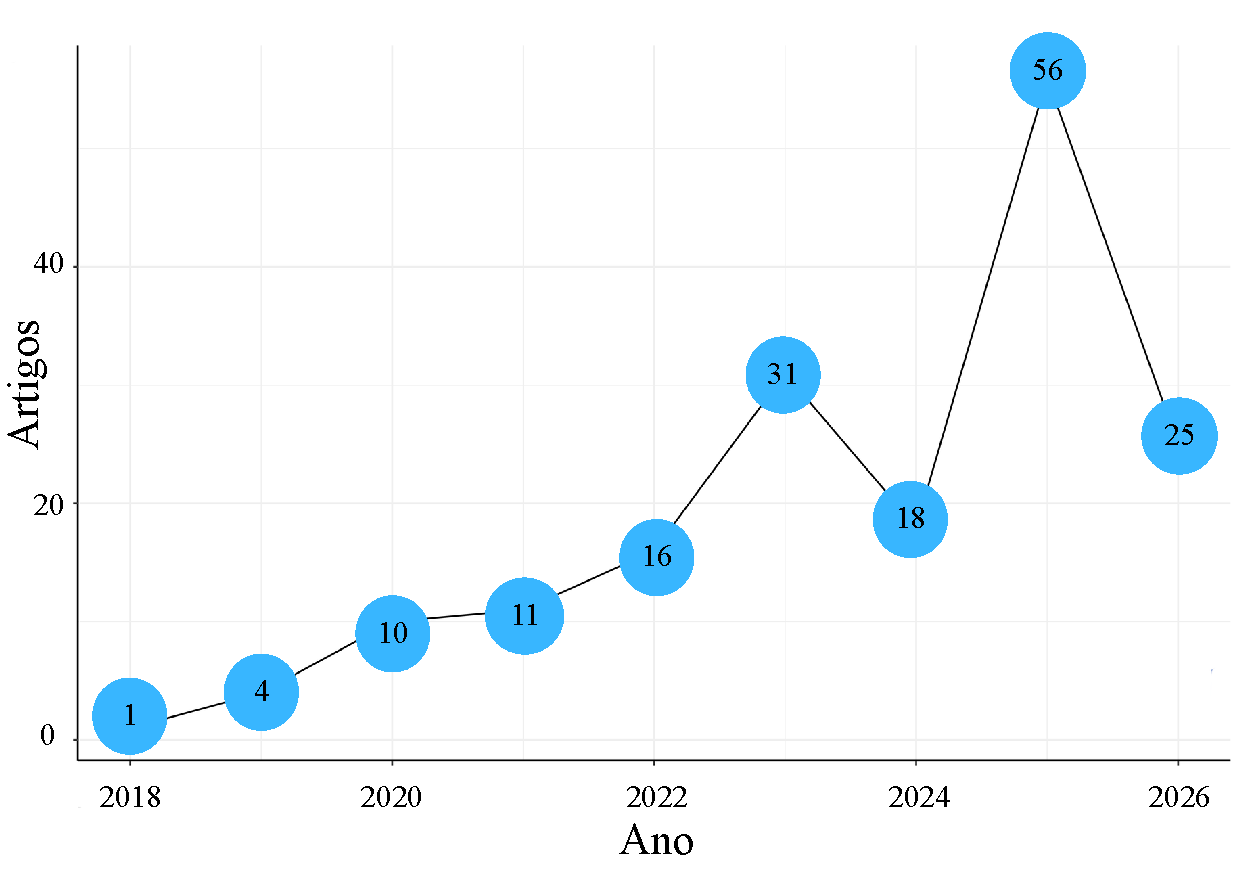
\includegraphics[height=5.7cm]{figuras/biblio_evolucao}
\begin{itemize} \footnotesize \itemsep0.25em
  \item Busca no \textbf{Scopus} (2018+) sobre ML aplicado à pecuária bovina: \textbf{172 documentos}, com crescimento e pico de 56 artigos em 2025.
\end{itemize}
\end{frame}

% ------------------------------------------------------------

\begin{frame}[fragile] \frametitle{Trabalhos Relacionados e Posicionamento}
\begin{itemize} \footnotesize \itemsep0.4em
  \item \textbf{Tuyishime \& Adewusi (2025)} \cite{tuyishime2025} -- predição do ganho de peso com variáveis zootécnicas, ambientais e de manejo; \emph{sem} variáveis sanitárias nem classificação.
  \item \textbf{Grzesiak et al. (2023)} \cite{grzesiak2023} -- classificação do GMD em categorias, porém com dados de linhagem materna (laboratoriais).
  \item \textbf{Bauer \& Jagusiak (2022)} \cite{bauer2022} -- MLP com retropropagação sobre variáveis sanitárias; valida a arquitetura adotada.
\end{itemize}
\vskip0.5em
\begin{block}{Diferencial deste trabalho}
\footnotesize Integra variáveis zootécnicas, \textbf{sanitárias}, climáticas e de manejo em um único modelo, com \textbf{dados de rotina} (sem câmeras/sensores) e classificação sem dados genômicos -- no recorte inédito de \textbf{Bambuí-MG}.
\end{block}
\end{frame}

% ------------------------------------------------------------

\subsection{Fundamentação Teórica}

\begin{frame}[fragile] \frametitle{Redes Neurais Artificiais (MLP)}
\begin{itemize} \itemsep0.7em
  \item RNAs são modelos inspirados no sistema nervoso biológico: neurônios organizados em camadas e interligados por conexões ponderadas \cite{mcculloch1943, rosenblatt1958}.
  \item Cada neurônio combina entradas e aplica uma função de ativação \cite{silva2016}:
    $$ y = f\!\left(\sum_{i=1}^{n} w_i x_i + b\right) $$
  \item \emph{Multilayer Perceptron} (MLP): camada de entrada (13 variáveis) $\rightarrow$ camadas ocultas (transformações não lineares) $\rightarrow$ saída com 1 neurônio linear \cite{goodfellow2016}.
  \item Ativação \textbf{ReLU} nas camadas ocultas ($f(x)=\max(0,x)$); saída \textbf{linear}, adequada ao GMD contínuo.
  \item Treinamento por retropropagação do erro e otimizador \textbf{Adam}.
\end{itemize}
\end{frame}

% ------------------------------------------------------------

\begin{frame}{Métricas de Avaliação}
\begin{columns}[t]
\begin{column}{0.46\linewidth}
  \begin{block}{Regressão (GMD contínuo)}
    \begin{itemize} \itemsep0.4em
      \item \textbf{MSE} -- penaliza fortemente erros grandes; sensível a outliers
      \item \textbf{RMSE} -- mesma unidade do GMD (kg/dia); mais interpretável
      \item \textbf{MAE} -- erro médio absoluto; menos sensível a outliers
    \end{itemize}
  \end{block}
\end{column}
\begin{column}{0.46\linewidth}
  \begin{block}{Classificação de desempenho}
    \begin{itemize} \itemsep0.4em
      \item GMD contínuo convertido em \textbf{3 classes}: baixo, médio e alto
      \item Limites por \textbf{quantis empíricos} (tercis: percentis 33,3\% e 66,7\%) $\rightarrow$ classes balanceadas
      \item Limiares estimados só no treino (evita vazamento)
      \item Métricas: \textbf{acurácia} e \textbf{F1-score}
    \end{itemize}
  \end{block}
\end{column}
\end{columns}
\end{frame}

% ------------------------------------------------------------

\begin{frame}[fragile] \frametitle{Variáveis do Conjunto de Dados}
\textbf{13 variáveis preditoras} em 5 grupos temáticos + variável-alvo:
\vskip0.5em
\begin{columns}[t]
\begin{column}{0.48\linewidth}
  \begin{itemize} \itemsep0.3em
    \item \textbf{Animal (3):} peso inicial, idade, proporção \emph{Bos indicus}
    \item \textbf{Nutrição/pastagem (5):} suplemento (quantidade, PB, EM), PB e digestibilidade da forragem
    \item \textbf{Manejo (1):} estresse por transporte
  \end{itemize}
\end{column}
\begin{column}{0.48\linewidth}
  \begin{itemize} \itemsep0.3em
    \item \textbf{Clima (2):} temperatura média, precipitação acumulada
    \item \textbf{Sanidade (2):} dias desde e duração do último evento sanitário
    \item \textbf{Alvo:} GMD (kg/dia)
  \end{itemize}
\end{column}
\end{columns}
\vskip0.6em
\footnotesize \textbf{Excluídas:} 5 variáveis de variância nula (condições homogêneas de manejo) e \texttt{dias\_permanencia} -- denominador do GMD, removida para evitar vazamento de informação.
\end{frame}

% ------------------------------------------------------------

\section{Metodologia}

\begin{frame}[fragile] \frametitle{Metodologia -- Coleta de Dados}
\begin{itemize} \itemsep0.7em
  \item Duas propriedades rurais da microrregião de \textbf{Bambuí-MG}, com autorização dos proprietários.
  \item Pesagens realizadas entre \textbf{2021 e 2026}; cada amostra corresponde a uma pesagem individual de um animal.
  \item Registros de controle interno transcritos para um formulário estruturado (\textbf{Google Forms}).
  \item Conjunto final: \textbf{494 amostras}.
  \item Limitações reconhecidas: independência das amostras (brinco reaproveitado entre animais) e leves variações de protocolo entre as fazendas.
\end{itemize}
\end{frame}

% ------------------------------------------------------------

\begin{frame}[fragile] \frametitle{Metodologia -- Pré-processamento e Variáveis}
\begin{columns}[t]
\begin{column}{0.48\linewidth}
  \begin{block}{Derivação automática}
    \begin{itemize} \itemsep0.3em
      \item GMD (alvo) pela fórmula do ganho
      \item Nutrição via tabelas \textbf{CQBAL}
      \item Clima via API \textbf{NASA POWER} (temperatura e precipitação)
    \end{itemize}
  \end{block}
\end{column}
\begin{column}{0.48\linewidth}
  \begin{block}{Tratamento e seleção}
    \begin{itemize} \itemsep0.3em
      \item Inconsistências, normalização e codificação de binárias
      \item Seleção por \textbf{literatura zootécnica}
      \item Remoção das 5 variáveis de variância nula e de \texttt{dias\_permanencia} (vazamento)
    \end{itemize}
  \end{block}
\end{column}
\end{columns}
\vskip0.6em
\footnotesize \textbf{Ferramentas:} Python, Pandas, PyTorch e Jupyter Notebook.
\end{frame}

% ------------------------------------------------------------

\section{Análise Exploratória}

\begin{frame}[fragile] \frametitle{Análise Exploratória -- Visão Geral}
\begin{itemize} \itemsep0.9em
  \item Conjunto de \textbf{494 amostras} e 20 variáveis, \textbf{sem valores ausentes} (coleta estruturada por formulário).
  \item 5 variáveis com valor \textbf{constante} (somente fêmeas, suplementação diária, pastejo rotacionado, sem vacinação/vermifugação recentes) -- mantidas fora dos preditores.
  \item Objetivo: caracterizar a variável-alvo e as preditoras \emph{antes} da modelagem.
\end{itemize}
\end{frame}

% ------------------------------------------------------------

\begin{frame}{Distribuição do Ganho Médio Diário}
\centering
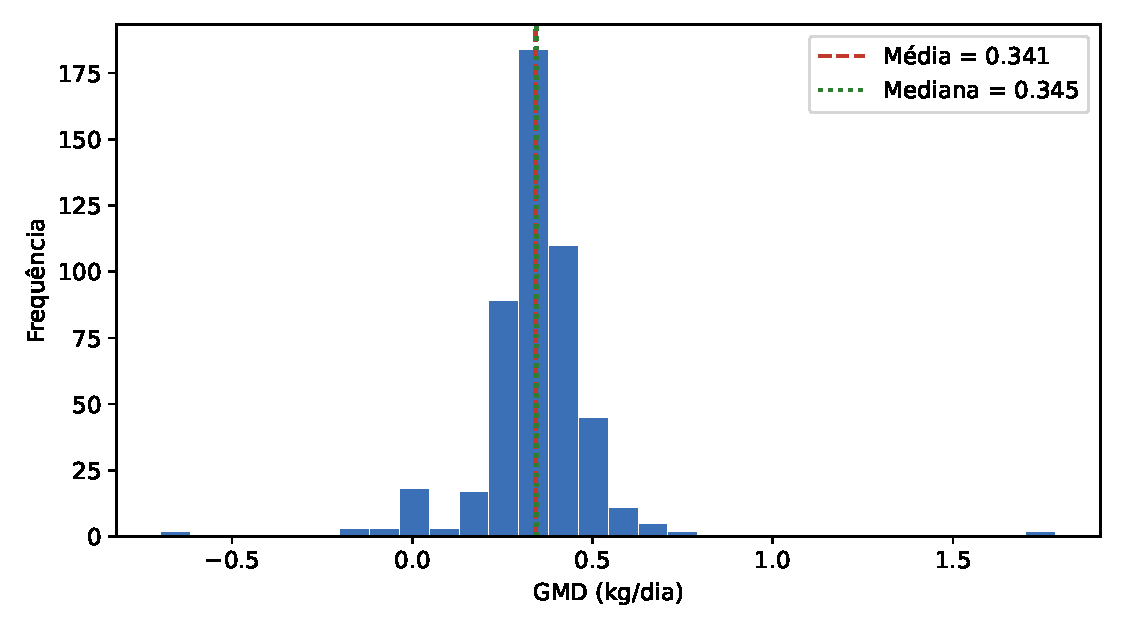
\includegraphics[height=5.2cm]{figuras/eda_gmd_dist}
\begin{itemize} \footnotesize \itemsep0.2em
  \item Média 0,341 e mediana 0,345 kg/dia.
  \item Valores negativos indicam perda de peso -- plausível a pasto na estação seca.
  \item Justifica definir as categorias por \textbf{quantis} (tercis), garantindo classes balanceadas.
\end{itemize}
\end{frame}

% ------------------------------------------------------------

\begin{frame}{Matriz de Correlação}
\centering
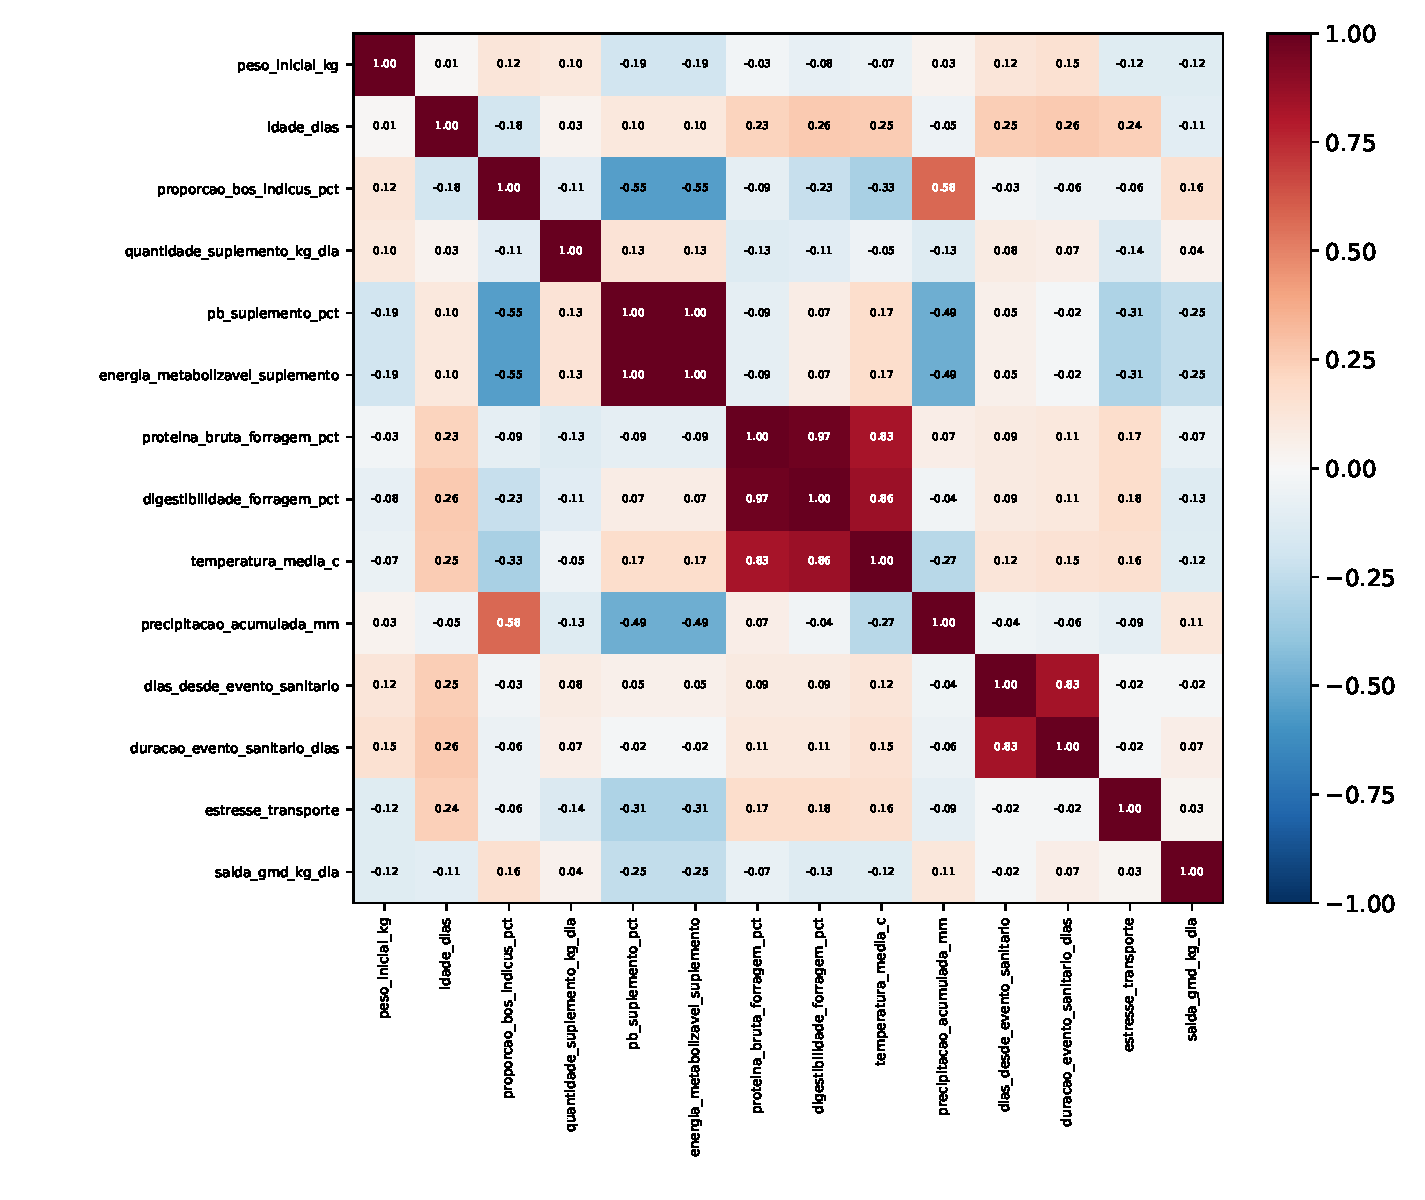
\includegraphics[height=6.1cm]{figuras/eda_corr_matrix}\\
{\footnotesize \textbf{Multicolinearidade} entre preditoras (ex.: PB e energia metabolizável; PB e digestibilidade da forragem).}
\end{frame}

% ------------------------------------------------------------

\begin{frame}{Correlação das Variáveis com o GMD}
\centering
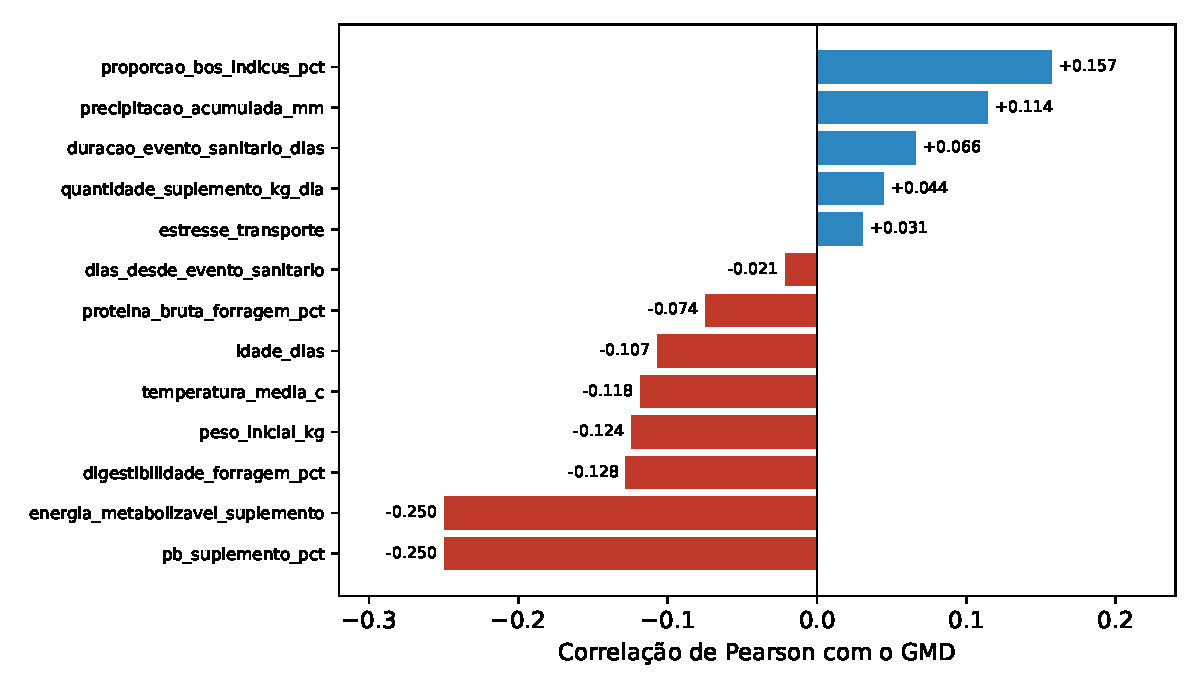
\includegraphics[height=5.1cm]{figuras/eda_corr_target}
\begin{itemize} \footnotesize \itemsep0.2em
  \item Todas as correlações lineares com o alvo são \textbf{fracas} ($|r| < 0{,}26$).
  \item Nenhuma variável isolada explica o GMD linearmente.
\end{itemize}
\end{frame}

% ------------------------------------------------------------

\section{Considerações Parciais}

\begin{frame}[fragile] \frametitle{Considerações Parciais e Próximos Passos}
\begin{columns}[t]
\begin{column}{0.5\linewidth}
  \begin{block}{Constatações}
    \begin{itemize} \itemsep0.3em
      \item Boa qualidade estrutural (sem faltantes; variáveis problemáticas identificadas)
      \item Alvo assimétrico com valores negativos $\rightarrow$ categorias por quantis
      \item Correlações fracas + multicolinearidade
    \end{itemize}
  \end{block}
\end{column}
\begin{column}{0.5\linewidth}
  \begin{block}{Próximos passos}
    \begin{itemize} \itemsep0.3em
      \item Treinamento e validação da MLP (busca de hiperparâmetros)
      \item Avaliação (MSE, RMSE, MAE) e classificação em categorias
      \item Ampliação da base com novas propriedades
    \end{itemize}
  \end{block}
\end{column}
\end{columns}
\end{frame}
% ------------------------------------------------------------



\section{Referências}

\begin{frame}[allowframebreaks]{Referências}
\footnotesize
\printbibliography
\end{frame}

\begin{frame}[fragile,plain] \frametitle{Obrigado}
\begin{center}
 \vspace*{2em}

 Favor enviar as sugestões e os pedidos de correção para eulergomesrocha@gmail.com.

 \vspace*{2em}
 
\includegraphics[width=1.5cm]{logoif}
\end{center}
\end{frame}

\end{document}
